\chapter{المؤشّرات (\textenglish{Pointers})}

لقد حان الوقت لنكتشف المؤشرات. خذ نفسا عميقا قبل أن تقرر قراءة هذا الفصل لأنه لن يكون فصلاً للهو و المرح. تمثل المؤشرات واحداً من المبادئ الأكثر أهمية و حساسية في لغة الـ\textenglish{C}
. و إن كنت أصرّ على أهميتها فهذا  لأنه لا يمكنك البرمجة بـ\textenglish{C}
دون معرفتها و فهمها جيّدا. المؤشرات موجودة في كلّ مكان، و لقد استعملتها من قبل دون أن تعلم بذلك.

كثير من المتعلّمين يصلون إلى المؤشرات و يواجهون صعوبات في فهمها. سنعمل على ألا يكون الأمر مماثلا بالنسبة لك. ضاعف التركيز و خذ الوقت اللازم لفهم المخططات التي سأقدمها لك في هذا الفصل.

\section{مشكل مضجر بالفعل}

واحد من أكبر المشاكل مع المؤشرات هي أنّه بالإضافة إلى أنها صعبة الاستيعاب قليلا بالنسبة للمبتدئين، فإن المتعلّم لا يعرف ما هي أهميتها و فيما يمكننا استعمالها.

يمكنني أن أقول لك بأن "المؤشرات لا يمكن الاستغناء عنها في أي برنامج
\textenglish{C}
، صدقني !"، لكنّي أعرف أن هذه الحجّة ليست كافية لك.

سأطرح عليك مشكلاً لا يمكنك حلّه إلا باستخدام المؤشرات. سيكون هذا الخيط الأحمر في هذا الفصل. سنعود إليه في نهاية هذا الفصل و سترى حلّه باستعمال ما تعلّمته في هذا الفصل.

إليك المشكل: أريد كتابة دالة تقوم بإرجاع قيمتين مختلفتين. ستجيبني "هذا مستحيل !". بالفعل، الدالة لا يمكنها إرجاع سوى قيمة واحدة.

\begin{Csource}
int function()
{
	return value;
}
\end{Csource}

إذا استخدمنا
\InlineCode{int}
ترجع لنا قيمة من نوع
\InlineCode{int}
(بفضل التعليمة
\InlineCode{return}).

يمكننا أيضا كتابة دالة لا تُرجع أية قيمة باستخدام الكلمة المفتاحية
\InlineCode{void}.

\begin{Csource}
void function()
{

}
\end{Csource}

لكن إرجاع قيمتين مختلفتين في نفس الوقت \dots هذا أمر مستحيل لأنه لا يمكننا استعمال تعليمتي
\InlineCode{return}.

لنفرض أنني أريد كتابة دالة أعطيها كمدخل عددا من الدقائق. تقوم الدالة بإرجاع عدد الساعات و الدقائق المواقفة لها.

\begin{itemize}
  \item إذا أعطيت القيمة 45  الدالة ترجع 0 ساعة و 45 دقيقة.
  \item إذا أعطيت القيمة 60 الدالة ترجع القيمة  1 ساعة و 0 دقائق.
	\item إذا أعطيت القيمة 90 الدالة ترجع القيمة  1 ساعة و 30 دقيقة.
\end{itemize}

لنكن مجانين و لنجرّب ذلك :

\begin{Csource}
#include <stdio.h>
#include <stdlib.h>

/* I put the prototype at the top.
Because it's a short code, I don't put it in a .h file.
In a real program I would have put the prototype
in a separate .h file of course */

void minutesDevision(int hours, int minutes);

int main(int argc, char *argv[])
{
	int hours = 0, minutes = 90;

/* We have a variable "minutes" equals to 90.
   after calling the function, I want from the variable
“hours" to take the value 1 and from my variable
"minutes" to take the value 30 */

	minutesDivision(hours, minutes);
	printf("%d hours and %d minutes", hours, minutes);
	return 0;
}

void minutesDevision(int hours, int minutes)
{
	hours = minutes / 60;  // 90 / 60 = 1
	minutes = minutes % 60; // 90 % 60 = 30
}
\end{Csource}

النتيجة :

\begin{Console}
0 hours and 90 minutes
\end{Console}

لم تشتغل ! ما الأمر يا ترى ؟
في الواقع، عندما نبعث متغيرا إلى دالة، يتم إنشاء نسخة من المتغير، و لهذا فالمتغير
\InlineCode{hours}
في الدالة
\InlineCode{minutesDevision}
هو ليس نفسه الذي في الدالة
\InlineCode{main} !
إنه فقط نسخة !

الدالة
\InlineCode{minutesDevision}
تقوم بعملها. ففي داخلها المتغيران
\InlineCode{hours}
و
\InlineCode{minutes}
يحملان القيمتين الصحيحتين : 1 و 30.

لكن بعد ذلك، تتوقف الدالة مباشرة عند الوصول إلى الحاضنة الغالقة، مثلما تعلمنا سابقا : المتغيرات الخاصة بدالة يتم حذفها مباشرة عند انتهاء الدالة. إذن النسخ عن المتغيرات
\InlineCode{minutes}
و
\InlineCode{hours}
تُمسح.
نرجع بعد ذلك للدالة
\InlineCode{main}.
و التي فيها متغيراتنا
\InlineCode{minutes}
و
\InlineCode{hours}
تحملان القيمتين 0 و 90. لقد فشلنا !

\begin{information}
	لاحظ إذن، بما أن الدالة تقوم بنسخ المتغيرات التي نعطيها لها، لست مضطراً لستمية متغيراتك بنفس الأسماء التي تحملها في الـدالة الرئيسية
\InlineCode{main}.
و بالتالي يمكنك ببساطة كتابة :

\InlineCode{void minutesDivision(int h, int m)}\\
\InlineCode{h}
للساعات و
\InlineCode{m}
للدقائق.\\
إن كانت متغيراتك لم تسمّى بنفس الطريقة في الدالة و في
\InlineCode{main}
فهذا لا يطرح أيّ مشكل !
\end{information}


باختصار، يمكنك إعادة المشكل في كلّ الاتجاهات. يمكنك محاولة بعث قيمة باستخدام الدالة (باستخدام
\InlineCode{return}
و باستخدام النوع
\InlineCode{int}
للدالة) ، لكن لا يمكنك إعادة أكثر من قيمة واحدة من بين القيمتين، هذا مشكل مطروح إذن. كما لا يمكنك استعمال متغيرات شاملة لأن هذا أمر غير مستحسن إطلاقا.

حسناً المشكل لازال مطروحاً، كيف يمكننا حلّه باستخدام المؤشرات ؟

\section{الذاكرة، مسألة عنوان}

\subsection{تذكير بالمكتسبات القبليّة}

سأعود بك قليلاً إلى الوراء، هل تتذكر فصل المتغيرات ؟

أيّا كانت إجابتك، أنصحك بأن تعود إلى ذلك الفصل و تقرأ منه القسم الذي يحمل عنوان (مسألة ذاكرة). هناك مخطط مهم جداً سأقترحه عليك من جديد :

\begin{figure}[H]
	\centering
	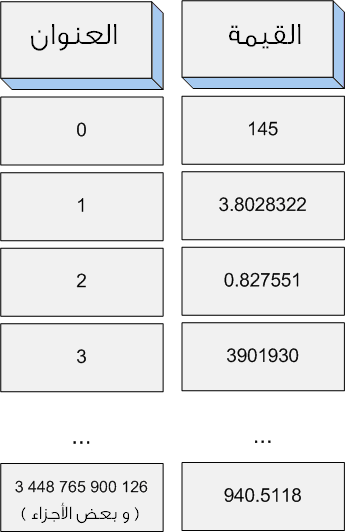
\includegraphics[width=0.4\textwidth]{Chapter_II-2_RAM-Schema}
\end{figure}


هكذا نقوم تقريباً بتمثيل الذاكرة الحية
(\textenglish{RAM})
الخاصة بالحاسوب.

يجب قراءة المخطط سطراً بسطر، السطر الأول يمثل "الخانة" الخاصة بأول الذاكرة. لكل خانة رقم، هذا الرقم يمثل
\textbf{عنوانها}
(تذكّر هذا المصطلح جيدا). تحتوي الذاكرة على عدد كبير جداً من العناوين تبدأ من الرقم 0 و تنتهي بالرقم
\textit{(ضع رقماً كبيراً جداً هنا)}.
عدد العناوين التي تتوفر عليها تعتمد على حجم الذاكرة التي يحتوي عليها الجهاز الخاص بك.

في كلّ عنوان يمكننا تخزين عدد واحد فقط. لا يمكننا تخزين عددين في نفس العنوان.

الذاكرة ليست مصنوعة سوى لتخزين الأعداد. لا يمكنها تخزين لا حروف و لا جُمل. و للتخلص من هذا المشكل تم اختراع جدول يقوم بالربط بين الحروف و الأعداد. يقول الجدول مثلاً :"العدد 89 يمثّل الحرف
\textenglish{Y}".
سنعود في فصل لاحق إلى كيفيّة معالجة الحروف. حاليّا، سنتكفي بالتكلّم عن عمل الذاكرة.

\subsection{عنوان و قيمة}

حينما تنشئ متغيراً
\InlineCode{age}
من نوع
\InlineCode{int}
مثلا، بكتابة :

\begin{Csource}
int age = 10;
\end{Csource}

يطلب البرنامج من نظام التشغيل (الويندوز مثلا) الإذن لاستعمال جزء من الذاكرة. نظام التشغيل يجيب بالإشارة إلى أي عنوان سيسمح لك بتخزين العدد.

هنا تكمن أحد أهم وظائف نظام التشغيل : نقول أنه يحجز الذاكرة للبرامج. يمكننا القول أنه هو القائد، يتحكم في كلّ برنامج و يتأكد من أن هذا الأخير له الإذن لاستعمال الذاكرة في المكان الذي يطلبه.

\begin{information}
إن هذا هو السبب الرئيسي في توقف البرامج عن العمل : إذا حاول برنامجك الوصول إلى مكان غير مسموح له بالوصول إليه في الذاكرة، سيرفض نظام التشغيل و يوقف تشغيله بشكل عنيف (لأنه القائد هنا). بينما يتلقّى المستعمل نافذة خطأ تحتوي على رسالة تشير بأن البرنامج يحاول القيام بعملية غير لائقة.
\end{information}

لنعد للمتغير
\InlineCode{age}.
تم تخزين القيمة 10 في مكان ما من الذاكرة، لنقل مثلاً في العنوان رقم 4655.\\
ما يحدث (و هذا دور المترجم) هو أن الكلمة
\InlineCode{age}
يتم تعويضها بالعنوان 4655 لحظة التنفيذ. مما يعني أنه في كلّ مرة قمت فيها بكتابة الكلمة
\InlineCode{age}
في الشفرة المصدرية، يتم تعوضيها بـ4655، و بهذا يرى الجهاز إلى أي عنوان في الذاكرة عليه الذهاب. و منه يجيب بكلّ فخر بأن المتغير
\InlineCode{age}
يحتوي القيمة 10.

نحن نعرف إذا كيف نسترجع قيمة متغير، يكفي بكلّ بساطة أن نكتب الكلمة
\InlineCode{age}
في الشفرة المصدرية. إذا أردنا إظهار السنّ، يمكننا استعمال الدالة
\InlineCode{printf} :

\begin{Csource}
printf("The value of variable age is : %d", age);
\end{Csource}

النتيجة على الشاشة :

\begin{Console}
The value of variable age is : 10
\end{Console}

لا شيء جديد لحدّ الآن.

\subsection{الخبر المثير لليوم}

أنت تعرف كيف تظهر قيمة متغير، لكن هل تعرف أنه بإمكاننا أيضا إظهار عنوانه ؟

لكي نُظهر عنوان متغير، نستعمل الإشارة
\InlineCode{\%p}
(الحرف
\textenglish{p}
مأخوذ من الكلمة
\textenglish{Pointer})
في الدالة
\InlineCode{printf}.
أي أننا لن نبعث للدالة
\InlineCode{printf}
المتغير في حدّ ذاته لكن نبعث لها عنوانه. و لفعل هذا، يجب عليك استعمال الإشارة
\InlineCode{\&}
أمام المتغير
\InlineCode{age}
كما طلبت منك أن تفعل مع الدالة
\InlineCode{scanf}
من قبل دون أن أشرح لك لماذا.

أكتب إذا:

\begin{Csource}
printf("The address of the variable age is  : %p", &age);
\end{Csource}
النتيجة :

\begin{Console}
The address of the variable age is : 0023FF74
\end{Console}

ما تراه هنا هو عنوان المتغير
\InlineCode{age}
في اللحظة التي طلبتُ فيها تنفيذ البرنامج من طرف حاسوبي. نعم نعم،
0023FF74
هو رقم، هو فقط مكتوب في النظام الست عشري
(\textenglish{Hexadecimal})
عوض النظام العشري الذي تعوّدنا عليه. لو تقوم بتعويض
\InlineCode{\%p}
بـ\InlineCode{\%d}
فإنه سيظهر لك رقما عشريا كما تعوّدنا.

\begin{information}
	إذا شغّلت البرنامج على حاسوبك فمن المؤكّد أن تحصل على عنوان آخر. الأمر يعتمد على المكان في الذاكرة، البرامج المشتغلة، إلخ.
فيستحيل أن تتوقع العنوان الّذي سيتم تخزين المتغيّر فيه.
إذا قمت بتشغيل البرنامج عدة مرات الواحدة تلو الأخرى قد تتحصل على نفس النتيجة كون الذاكرة لم تتغير في ذلك الزمن القصير.
لكن بالمقابل إن أعدت تشغيل الحاسوب فستتحصل بكل تأكيد على نتائج مختلفة.
\end{information}

إلى أين أريد الوصول بكلّ هذا ؟ أريدك أن تتذكّر التالي :

\begin{itemize}
	\item \InlineCode{age} : تعني قيمة المتغير.
	\item \InlineCode{\&age} : تعني عنوان المتغير.
\end{itemize}

عند استخدام
\InlineCode{age}
سيقرأ الحاسوب قيمة المتغيّر في الذاكرة. أمّا عند استخدام
\InlineCode{\&age}
فسيعيد العنوان الذي يوجد فيه المتغيّر.

\section{استعمال المؤشرات}

لحدّ الآن، قمنا فقط بإنشاء متغيرات تحتوي على أعداد. الآن سنتعلّم كيف ننشئ متغيرات تحتوي على عناوين : هذا ما نسميه بالمؤشرات.

\begin{question}
	لكن \dots العناوين هي أعداد أيضاً، أليس كذلك ؟ هذا يعني أننا سنخزن أعداداً دائما !
\end{question}

هذا صحيح، لكن لهذه الأعداد معنى آخر : هي تشير إلى عنوان متغير آخر في الذاكرة.

\subsection{إنشاء مؤشّر}

لإنشاء متغير من نوع مؤشّر، يجب علينا أن نضيف الرمز
\InlineCode{*}
أمام إسم المتغير :

\begin{Csource}
int *myPointer;
\end{Csource}

\begin{information}
لاحظ أنه يمكننا أيضا أن نكتب
\InlineCode{int* myPointer;}
لهذا نفس المعنى. لكن الطريقة الأولى هي المفضّلة. في الواقع، إن كنت تريد التصريح عن العديد من المؤشرات في نفس السطر، سيكون عليك أن تعيد كتابة النجمة أمام كل اسم :
\InlineCode{int *pointer1, *pointer2, *pointer3;}
\end{information}

كما قلت لك، من المهمّ أن تقوم بإعطاء قيم إبتدائية للمتغيرات منذ البداية، و ذلك بإعطائها القيمة 0 مثلا~! إنه من المهم أكثر أن تفعل نفس الشيء مع المؤشرات.\\
لتهيئة مؤشّر، نعطيه قيمة افتراضية، لا نستعمل غالبا القيمة 0 و لكن الكلمة المفتاحية
\InlineCode{NULL}
(أكتبها بأحرف كبيرة).

\begin{Csource}
int *myPointer = NULL;
\end{Csource}

هنا لدينا مؤشر يحمل القيمة الإبتدائية
\InlineCode{NULL}.
هكذا ستعرف لاحقاً في البرنامج أن المؤشر لا يحتوي على أي عنوان.

ما الذي يحصل ؟ ستقوم هذه الشفرة المصدرية بحجز خانة في الذاكرة كما لو أننا أنشأنا متغيراً عادياً. الشيء الذي يتغير هو أن المؤشر سيحتوي عنوانا. عنوان متغير آخر.

لم لا عنوان المتغير
\InlineCode{age}
؟ أنت تعرف الآن كيف تشير إلى عنوان متغير في مكان قيمته (باستعمال الرمز
\InlineCode{\&})،
هيا بنا إذن ! هذا ما عليك كتابته :

\begin{Csource}
int age = 10;
int *PointerOnAge = &age;
\end{Csource}

السطر الأول يعني : "أنشئ متغيرا من نوع
\InlineCode{int}
يحمل القيمة 10". السطر الثاني يعني "أنشئ متغيراً من نوع مؤشّر قيمته هي عنوان المتغير
\InlineCode{age}".

يقوم إذا السطر الثاني بمهمّتين معاً. لكي لا تختلط عليك الأمور، إعلم أنه يمكننا تقسيم السطر إلى سطرين :

\begin{Csource}
int age = 10;
int *PointerOnAge; // 1) Means "I create the pointer"
PointerOnAge = &age; // 2) Means the pointer "PointerOnAge contains the address of age"
\end{Csource}

يمكنك الملاحظة أنه لا يوجد في لغة الـ\textenglish{C}
نوع نسميه
\InlineCode{pointer}
كالنوع
\InlineCode{int}
و
\InlineCode{double}.
أي أنه لا يمكننا أن نكتب :

\begin{Csource}
pointer PointerOnAge;
\end{Csource}

في مكان هذا، نستعمل الرمز
\InlineCode{*}
، و لكن نستمر في كتابة
\InlineCode{int}.
ماذا يعني هذا ؟ في الواقع يجب أن نشير إلى نوع المتغير الذي سيحوي عنوانه المؤشر. بما أن المؤشر
\InlineCode{PointerOnAge}
سيحتوي عنوان المتغير
\InlineCode{age}
(الذي هو من نوع
\InlineCode{int})،
إذا فالمؤشر يجب أن يكون من نوع
\InlineCode{int*}
! إذا كان المتغير من نوع
\InlineCode{double}
فإنه يجب عليّ أن أكتب
\InlineCode{double *myPointer}.

\textbf{إصطلاح}
: نقول بأن المؤشّر
\InlineCode{PointerOnAge}
يؤشّر على المتغير
\InlineCode{age}.

المخطط التالي يلخّص ما يحصل في الذاكرة :

\begin{figure}[H]
	\centering
	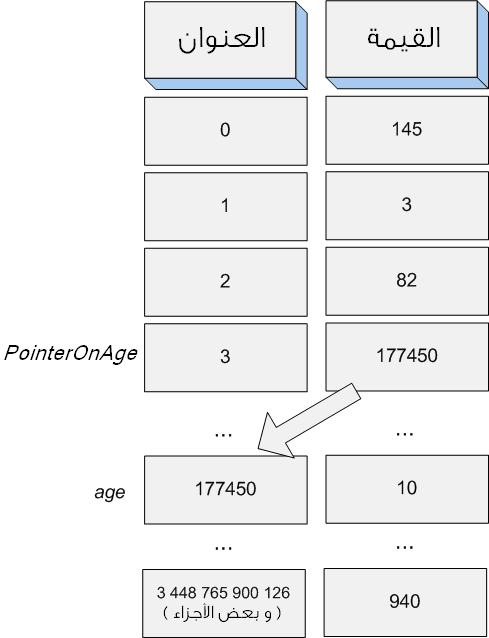
\includegraphics[width=0.5\textwidth]{Chapter_II-2_RAM-Schema-Pointer}
\end{figure}

في هذا المخطط، تم تعويض المتغير
\InlineCode{age}
بالعنوان 177450 (أنت ترى بأن قيمته هي 10)، و المؤشّر
\InlineCode{PointerOnAge}
تم تعويضه بالعنوان 3 (هذه محض صدفة).

حينما يتم إنشاء المؤشر، يقوم نظام التشغيل بحجز خانة في الذاكرة كما فعل مع المتغير
\InlineCode{age}.
الشيء المختلف هنا هو أن المتغير
\InlineCode{PointerOnAge}
له معنى آخر. أنظر للمخطط جيداً : قيمته هي عنوان المتغير
\InlineCode{age}.

هذا، عزيزي القارئ، هو السرّ المطلق من وراء كتابة البرامج في لغة الـ\textenglish{C}.
بهذا نحن ندخل في عالم المؤشرات العجيب !
\begin{question}
	و \dots ما هي فائدة هذا ؟
\end{question}
هذا لا يقوم بتحويل الحاسوب إلى آلة صنع القهوة، طبعا. لكن الآن لدينا المؤشر
\InlineCode{PointerOnAge}
يحتوي عنوان المتغير
\InlineCode{age}.

فلنحاول رؤية ما يحتويه المؤشر بالإستعانة بالدالة
\InlineCode{printf} :
\begin{Csource}
int age = 10;
int *PointerOnAge = &age;
printf("%d", PointerOnAge);
\end{Csource}
\begin{Console}
177450
\end{Console}
هذا ليس مفاجئاً، نحن نطلب قيمة
\InlineCode{PointerOnAge}
و قيمته هي عنوان المتغير
\InlineCode{age}
(أي 177450).\\
ماذا نفعل لكي نطلب قيمة المتغير المتواجدة في العنوان الذي يشير إليه المؤشّر
\InlineCode{PointerOnAge}
؟ يجب أن نضع الرمز
\InlineCode{*}
أمام إسم المؤشّر :
\begin{Csource}
int age = 10;
int *PointerOnAge = &age;
printf("%d, *PointerOnAge);
\end{Csource}
\begin{Console}
10
\end{Console}
ها قد وصلنا ! بوضع الرمز
\InlineCode{*}
أمام إسم المؤشّر، يمكننا الوصول إلى قيمة المتغير
\InlineCode{age}.

لو استعملنا الرمز
\InlineCode{\&}
أمام اسم المؤشّر، سنتحصل على العنوان الذي يتواجد به المؤشّر (هنا الرقم 3).

\begin{question}
	ماذا نربح هنا ؟ لقد نجحنا في تعقيد الأمور لا أكثر. لم نكن نحتاج إلى مؤشّر لنظهر قيمة المتغير
\InlineCode{age} !
\end{question}

هذا السؤال (الذي لا مفر من طرحه) شرعي، حاليّا الهدف ليس واضحا، لكن شيئاً فشيئاً، و مع تقدّم الفصول، ستفهم بأن كلّ هذه المبادئ لم يتم اختراعها من أجل تعقيد الأمور بكلّ سذاجة.

المهم هو أن تفهم المبدأ الآن و بعده ستتوضح الأمور لوحدها رويداً رويداً.

\subsection{ما يجب تذكّره}

هذا ما يفترض أن تكون قد فهمته و يجب عليك تذكره لباقي الفصل :

\begin{itemize}
	\item بالنسبة لمتغير كالمتغير
\InlineCode{age} :
	\begin{itemize}
		\item \InlineCode{age} تعني: "أريد قيمة المتغير
\InlineCode{age}"
		\item \InlineCode{\&age}
تعني: "أريد العنوان الذي يتواجد به المتغير
\InlineCode{age}"
	\end{itemize}
	\item بالنسبة لمؤشّر كالمؤشر
\InlineCode{PointerOnAge} :
	\begin{itemize}
		\item \InlineCode{PointerOnAge}
تعني: "أريد قيمة
\InlineCode{PointerOnAge}"
(هذه القيمة هي عنوان).
		\item \InlineCode{*PointerOnAge}
تعني : "أريد قيمة المتغير المتواجد في العنوان الذي يحتويه المؤشر
\InlineCode{PointerOnAge}".
	\end{itemize}
\end{itemize}

اكتفِ بفهم و حفظ النقاط الأربع السابقة، قم باختبارات و تأكد أنها تعمل. المخطط التالي سيعينك على فهم هذه النقاط :

\begin{figure}[H]
	\centering
	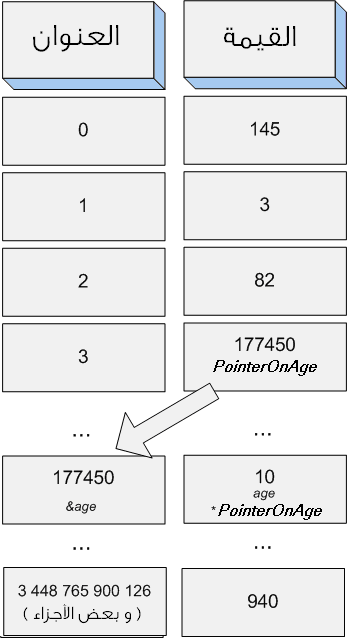
\includegraphics[width=0.4\textwidth]{Chapter_II-2_RAM-Schema-Pointer2}
\end{figure}


\begin{warning}
احذر في عدم الخلط بين مختلف تفسيرات النجمة ! حينما تصرّح عن مؤشّر، فّإن النجمة تشير إلى أننا بصدد إنشاء مؤشر :
\InlineCode{int *PointerOnAge;}
بينما لما نكتبها بجانب اسم المؤشر بكتابة~:
\InlineCode{printf("\%d", *PointerOnAge);}
فهذا يعني : أريد قيمة المتغير التي يشير إليها المؤشر
\InlineCode{PointerOnAge}.
\end{warning}

كل هذه المعلومات مبدئية. يجب أن تعرفها و الأهمّ أن تتعلّمها عن ظهر قلب. لا تتردّد في قراءة و إعادة قراءة ما قدّمته لك. لا يمكنني أن أعاتبك إذا لم تفهم من المرّة الأولى، و هذا ليس أمرا مخجلا. عادة ما تحتاج لعدّة أيّام لكي تفهمها جيّدا و بضعة شهور لتفهم كلّ شيء.

إذا كنت تشعر بأنك ضائع قليلاً، فكر في الأشخاص المحترفين في البرمجة : لا أحد منهم فهم مبدأ عمل المؤشرات من المرّة الأولى. و إن كان هذا الشخص موجوداً، أطلب منك أن تقدّمه لي الآن.

\section{إرسال مؤشّر إلى دالة}
أهم فائدة للمؤشرات (لكنها ليست الوحيدة) هي أنه بامكاننا إرسالها إلى دالة كي تقوم بتعديل مباشر على قيمة متغير في الذاكرة لا لنسخة منها كما رأينا سابقاً.

كيف يعمل هذا ؟ هناك الكثير من الطرق لفعل هذا. إليك مثالاً :
\begin{Csource}
void triplePointer(int *numberPointer);

int main(int argc, char *argv[])
{
	int number = 5;

	triplePointer(&number); // We send the address of number to the function
	printf("%d", number); // We display the variable number. The function has directly modified its value because it knows the address of the variable

	return 0;
}

void triplePointeur(int *numberPointer)
{
	*numberPointer *= 3; // We multiply by 3 the value of number
}
\end{Csource}
\begin{Console}
15
\end{Console}
الدالة
\InlineCode{triplePointer}
تأخذ معاملا من نوع
\InlineCode{int*}
(أي مؤشّر على
\InlineCode{int}).\\
إليك ما يحدث بالترتيب، إنطلاقاً من بداية الدالة
\InlineCode{main} :
\begin{enumerate}
	\item يتم إنشاء متغير
\InlineCode{number}
في الدالة
\InlineCode{main}،
نُسنِد له القيمة 5، أنت تعرف هذا.
	\item نستدعي الدالة
\InlineCode{triplePointer}
و نرسل لها كمعامل عنوان المتغير
\InlineCode{number}.
	\item تتلقّى الدالة
\InlineCode{triplePointer}
المتغير في المؤشر
\InlineCode{numberPointer}.
داخل الدالة\\
\InlineCode{triplePointer}،
لدينا إذن المؤشر
\InlineCode{numberPointer}
الذي يؤشر على المتغير
\InlineCode{number}.
	\item و الآن بما أنه لدينا مؤشر على المتغير
\InlineCode{number}،
يمكننا تغيير قيمة المتغير
\InlineCode{number}
مباشرة في الذاكرة~! يكفي استعمال
\InlineCode{numberPointer*}
للإشارة إلى المتغير
\InlineCode{number} !
كمثال، نقوم باختبار بسيط : نضرب المتغير في 3.
	\item يالعودة إلى
\InlineCode{main}،
يحتوي المتغير
\InlineCode{number}
القيمة 15 لأن الدالة
\InlineCode{triplePointer}
قامت بتعديل قيمته مباشرة.
\end{enumerate}

بالطبع، كان بإمكاني استعمال
\InlineCode{return}
بسيط كما تعلمنا القيام بذلك في الفصل الخاص بالدوال. لكن الهدف هنا، هو أنه بهذه الطريقة، أي باستعمال المؤشرات، يمكننا تعديل قيم الكثير من المتغيرات في الذاكرة (يمكننا إذا "إرجاع" الكثير من القيم !). لسنا محدودين بقيمة واحدة بعد الآن !

\begin{question}
	ما الفائدة الآن من استعمال
\InlineCode{return}
في دالة إذا كان بإمكاننا استعمال المؤشرات لتعديل قيم المتغيرات~؟
\end{question}

هذا يعتمد عليك و على برنامجك. القرار لك. يجب أن تعرف أن تعليمة
\InlineCode{return}
مستعملة بكثرة في لغة الـ\textenglish{C}.
غالباً نستعملها لإرجاع شفرة الخطأ : الدالة ترجع القيمة 1 (صحيح) إذا اشتغل كل شيء على ما يُرام، و 0 (خطأ) إذا حدث خطأ ما أثناء تشغيل البرنامج.

\subsection{طريقة أخرى لإرسال مؤشر إلى دالة}
في الشفرة المصدرية التي رأيناها، لم يكن هناك مؤشر في الدالة
\InlineCode{main}،
و إنما فقط متغير
\InlineCode{number}.
المؤشر الوحيد كان في الدالة
\InlineCode{triplePointer}
(من نوع
\InlineCode{int*}).

يجب أن تعرف أنه هناك طريقة أخرى لكتابة الشفرة المصدرية السابقة، وذلك بإضافة مؤشر في الدالة
\InlineCode{main} :

\begin{Csource}
void triplePointer(int *numberPointer);

int main(int argc, char *argv[])
{
	int number = 5;
	int *pointer = &number; // pointer gets the address of number
	triplePointer(pointer); // We send pointer (the address of number) to the function
	printf("%d", *pointeur);
	return 0;
}

void triplePointer(int *numberPointer)
{
	*numberPointer *= 3; // We multiply by 3 the value of number
}
\end{Csource}

قارن بين الشفرتين المصدريتين السابقتين، ستجد بأن هناك اختلافا بينهما، لكن النتيجة واحدة :

\begin{Console}
15
\end{Console}

ما يهم، هو بعث عنوان المتغير
\InlineCode{number}
إلى الدالة. لكن المؤشر يحمل عنوان المتغير
\InlineCode{number}،
فهذا جيد من هذه الناحية ! نحن فقط نقوم بالأمر بطريقة مختلفة بإنشاء المؤشر في الدالة
\InlineCode{main}.\\
في الدالة
\InlineCode{printf}
(فقط من أجل التمرين)، أُظهر محتوى المتغير
\InlineCode{number}
بكتابة
\InlineCode{*pointer}.
لاحظ أنه في مكان هذا، يمكنني كتابة
\InlineCode{number}
: ستكون النتيجة هي نفسها لأنّ
\InlineCode{*pointer}
و
\InlineCode{number}
يشيران إلى نفس الخانة بالذاكرة.

في البرنامج "أكثر أو أقل"، استعملنا مؤشراً دون أن نعرف بذلك. كان ذلك عند استدعاء الدالة
\InlineCode{scanf}.
بالفعل، دور هذه الدالة هو قراءة ما كتبه المستعمل في لوحة المفاتيح و إرجاع النتيجة. لكي تتمكن الدالة من تغيير محتوى المتغير مباشرة أي تضع بها الكلمة أو الجملة التي تمت كتابتها في لوحة المفاتيح، احتاجت لعنوان المتغير~:

\begin{Csource}
int number = 0;
scanf("%d", &number);
\end{Csource}

تعمل الدالة بمؤشر على المتغير
\InlineCode{number}
و بهذا يمكنها تغيير قيمته مباشرة.\\
كما رأينا الآن، يمكننا إنشاء مؤشر و نبعثه للدالة
\InlineCode{scanf} :

\begin{Csource}
int number = 0;
int *pointer = &number;
scanf("%d", pointer);
\end{Csource}

إنتبه كي لا تضع الرمز
\InlineCode{\&}
امام اسم مؤشر في الدالة
\InlineCode{scanf} !
هنا
\InlineCode{pointer}
يحتوي هو نفسه عنوان المتغير
\InlineCode{number}،
لذا أنت لا تحتاج لوضع
\InlineCode{\&} !
إذا فعلت هذا فإنك ستبعث العنوان الذي يتواجد به المؤشر : و لكننا بحاجة لعنوان
\InlineCode{number} !

\section{من الذي قال "مشكل مضجر بالفعل" ؟}

اقتربنا من نهاية الفصل، حان الوقت لإيجاد الخيط الأحمر. إذا كنت قد فهمت الفصل، فأنت قادر على حلّ المشكل. الآن، ما الذي تقوله. حاول حل المشكل و إليك الحل للمقارنة :

\begin{Csource}
void minutesDivision(int* hoursPointer, int* minutesPointer);

int main(int argc, char *argv[])
{
	int hours = 0, minutes = 90;
	// We send the addresses of hours and minutes
	minutesDivision(&hours, &minutes);
	// This time, the values are modified !
	printf("%d hours and %d minutes", hours, minutes);
	return 0;
}

void minutesDivision(int* hoursPointer, int* minutesPointer)
{
	/* Don't forget to put a star next to the pointer's name ! so you can modify the value of the variable and not its address ! You don't want to divide addresses, do you ? */
	*hoursPointer = *minutesPointer / 60;
	*minutesPointer = *minutesPointer % 60;
}
\end{Csource}

النتيجة :

\begin{Console}
1 hours and 30 minutes
\end{Console}

لا شيء يجب أن يفاجئك في هذه الشفرة المصدرية. كما أفعل في كلّ مرة، سأشرح ما يحصل هنا خطوة بخطوة لأتأكد من أن جميع القرّاء قد فهموا المبدأ. إنه فصل مهم و لهذا عليك أن تبذل حهدا كبيراً لتفهم كما أفعل أنا من أجلك~!

\begin{itemize}
	\item يتم إنشاء المتغيرين
\InlineCode{hours}
و
\InlineCode{minutes}
في الدالة
\InlineCode{main}.
	\item نرسل للدالة
\InlineCode{minutesDevision}
عنواني المتغيرين
\InlineCode{hours}
و
\InlineCode{minutes}.
	\item تقوم الدالة
\InlineCode{minutesDevision}
باسترجاع قيمتي المتغيرين في مؤشرين يدعيان
\InlineCode{hoursPointer}
و
\InlineCode{minutesPointer}.
لاحظ أنه لا يهم الاسم هنا أيضاً. كان بإمكاني تسميتهما
\InlineCode{m}
و
\InlineCode{h}،
أو حتى
\InlineCode{hours}
و
\InlineCode{minutes}
لم أقم بهذا لكي لا تخلط بين المتغيرين الخاصين بالدالة الرئيسية مع هذين المؤشرين اللذان يختلفان معهما.
	\item تقوم الدالة
\InlineCode{minutesDivision}
بتعديل مباشر لقيمتي المتغيرين
\InlineCode{hours}
و
\InlineCode{minutes}
في الذاكرة لأنها تملك عنوانيهما في مؤشرين. الشيء الوحيد الذي يمكنه أن يشكل مشكلا و يجب أن أبقيه ببالي هو وضع النجمة أمام اسمي المؤشرين إذا أردت أن أغير قيمتي المتغيرين
\InlineCode{hours}
و
\InlineCode{minutes}.
إذا لم نفعل هذا، فإننا سنغير العنوانين الموجودين في المؤشرين، و هذا لا ينفع في شيء.
\end{itemize}

\begin{information}
	كثير من القرّاء سيشيرون إلى أنه يمكن حل المشكل دون اللجوء إلى المؤشرات. نعم هذا صحيح، لكنّ هذا سيضطرنا لتجاوز القواعد التي وضعناها معاً. يمكننا استعمال المتغيرات الشاملة (و كما قلتُ هذا شيء سيء)، و يمكننا أيضاً وضع الدالة
\InlineCode{printf}
داخل الدالة
\InlineCode{minutesDivision}
(لكننا نحن نريد وضع العرض في الدالة الرئيسية). هذا يعني أنه يمكننا دائما حل المشكل باعتماد طرق غير لائقة مما يجعلك تشك في الفائدة من المؤشرات. لكن تأكد من أنك ستجد بأن استعمال المؤشرات أمر بديهي مع التقدم في الكتاب.
\end{information}

\section*{ملخّص}

\begin{itemize}
	\item كل متغير يتم تخزينه في
\textbf{عنوان}
معين من الذاكرة.
	\item تشبه
\textbf{المؤشرات}
المتغيرات لكنها مخصصة لتخزين العناوين التي تتواجد بها المتغيرات في الذاكرة.
	\item إذا وضعنا الرمز
\InlineCode{\&}
أمام اسم متغير فإننا نتحصل على العنوان الذي يتواجد به المتغير، مثلا :
\InlineCode{\&age}.
	\item إذا وضعنا الرمز
\InlineCode{*}
امام إسم مؤشر نتحصل على قيمة المتغير التي يؤشّر عليها المؤشّر.
	\item تعتبر المؤشرات إحدى المبادئ الأساسية في لغة الـ\textenglish{C}، تبدو صعبة في البداية لكن عليك أن تفهمها لأن الكثير من المبادئ الأخرى تقوم عليها.
\end{itemize}
